 \chapter{Metodologia de pesquisa}

Segundo \citeonline[pág.~2]{rodrigues2007}, a pesquisa deve conter um conjunto de abordagens, técnicas e processos para formular e resolver problemas do mundo real de maneira organizada e sistemática.

Para que uma pesquisa fique bem estruturada é necessário responder como os objetivos serão alcançados e  como será realizada a resolução do problema de pesquisa. Para isso, deve-se classificar a pesquisa, identificar as atividades e estabelecer como as atividades serão executadas \cite{forcon2014}.

\section{Classificação da Pesquisa}

Segundo \citeonline[pág.~41]{gil2008}, a metodologia de pesquisa é classificada através de critérios bem definidos com base em seus objetivos e procedimentos técnicos.

É usual classificar uma pesquisa com base em seus objetivos em três grandes grupos: exploratórias, descritivas e explicativas. Já em nível de procedimento técnico, a pesquisa pode ser classificada como estudo de caso, pesquisa-ação, survey, experimental, entre outras \cite[pág.~41]{gil2008}.

A pesquisa exploratória é utilizada pelo pesquisador para se familiarizar com um assunto pouco explorado. Ao decorrer ou no final da pesquisa exploratória, o pesquisador poderá estar apto para formular hipóteses \cite{giudice}.

A pesquisa descritiva é usada quando se tem um conhecimento do assunto e se quer descrever um fenômeno. Hipóteses podem ser formuladas com base em conhecimentos prévios, procurando confirmá-las ou negá-las \cite[pág.~21]{fonseca2002}.

A pesquisa é classificada com base em procedimentos técnicos, podendo ser quantitativa ou qualitativa. A pesquisa quantitativa traduz em números os estudos realizados e se utiliza técnicas estatísticas para comprovar os fatos \cite[pág.~9]{rodrigues2007}


As pesquisas atuais revelam que o reconhecimento mútuo e integração das abordagens qualitativas e quantitativas já é reconhecido \cite{serapioni}.

O estudo de caso é um estudo profundo, recomendável para temas muito complexos, em que é muito dificil gerar generalizações \cite[pág.~33]{fonseca2002}.

O estudo de caso vem sendo utilizado tanto em pesquisas exploratórias quanto descritivas e explicativas. É de sua natureza adotar na maioria dos casos, uma abordagem qualitativa, mas nada impede que o estudo de caso trabalhe com abordagens quantitativas \cite[pág.~22]{yin}.

Considerando os objetivos de estudo deste trabalho, foi incorporada uma pesquisa exploratória com o intuito de evidenciar os possíveis fenômenos que se repetem no mercado de moedas e uma pesquisa descritiva para evidenciar os benefícios da abordagem multiparadigma do software InvestMVC e da qualidade de código tanto a nível de testes unitários quanto a nível de análise estática de código.

Em relação aos procedimentos técnicos, foi utilizado o estudo de caso, pois apesar deste trabalho ter uma abordagem quantitativa dos dados e envolvimento de Métodos Matemáticos para elaboração de estratégias, não é possível afirmar que os resultados podem ser generalizados para outros contextos, como por exemplo, para a bolsa de valores ou até mesmo um par de moedas diferente do euro-dólar.

\section{Atividades da Pesquisa}

É necessário evidenciar na metodologia de pesquisa quando começam as atividades e quais são as coordenadas para que as mesmas sejam cumpridas \cite{forcon2014}.

A Figura \ref{metodologia} evidencia como foram organizadas as atividades deste trabalho.

\begin{figure}[H]
\centering
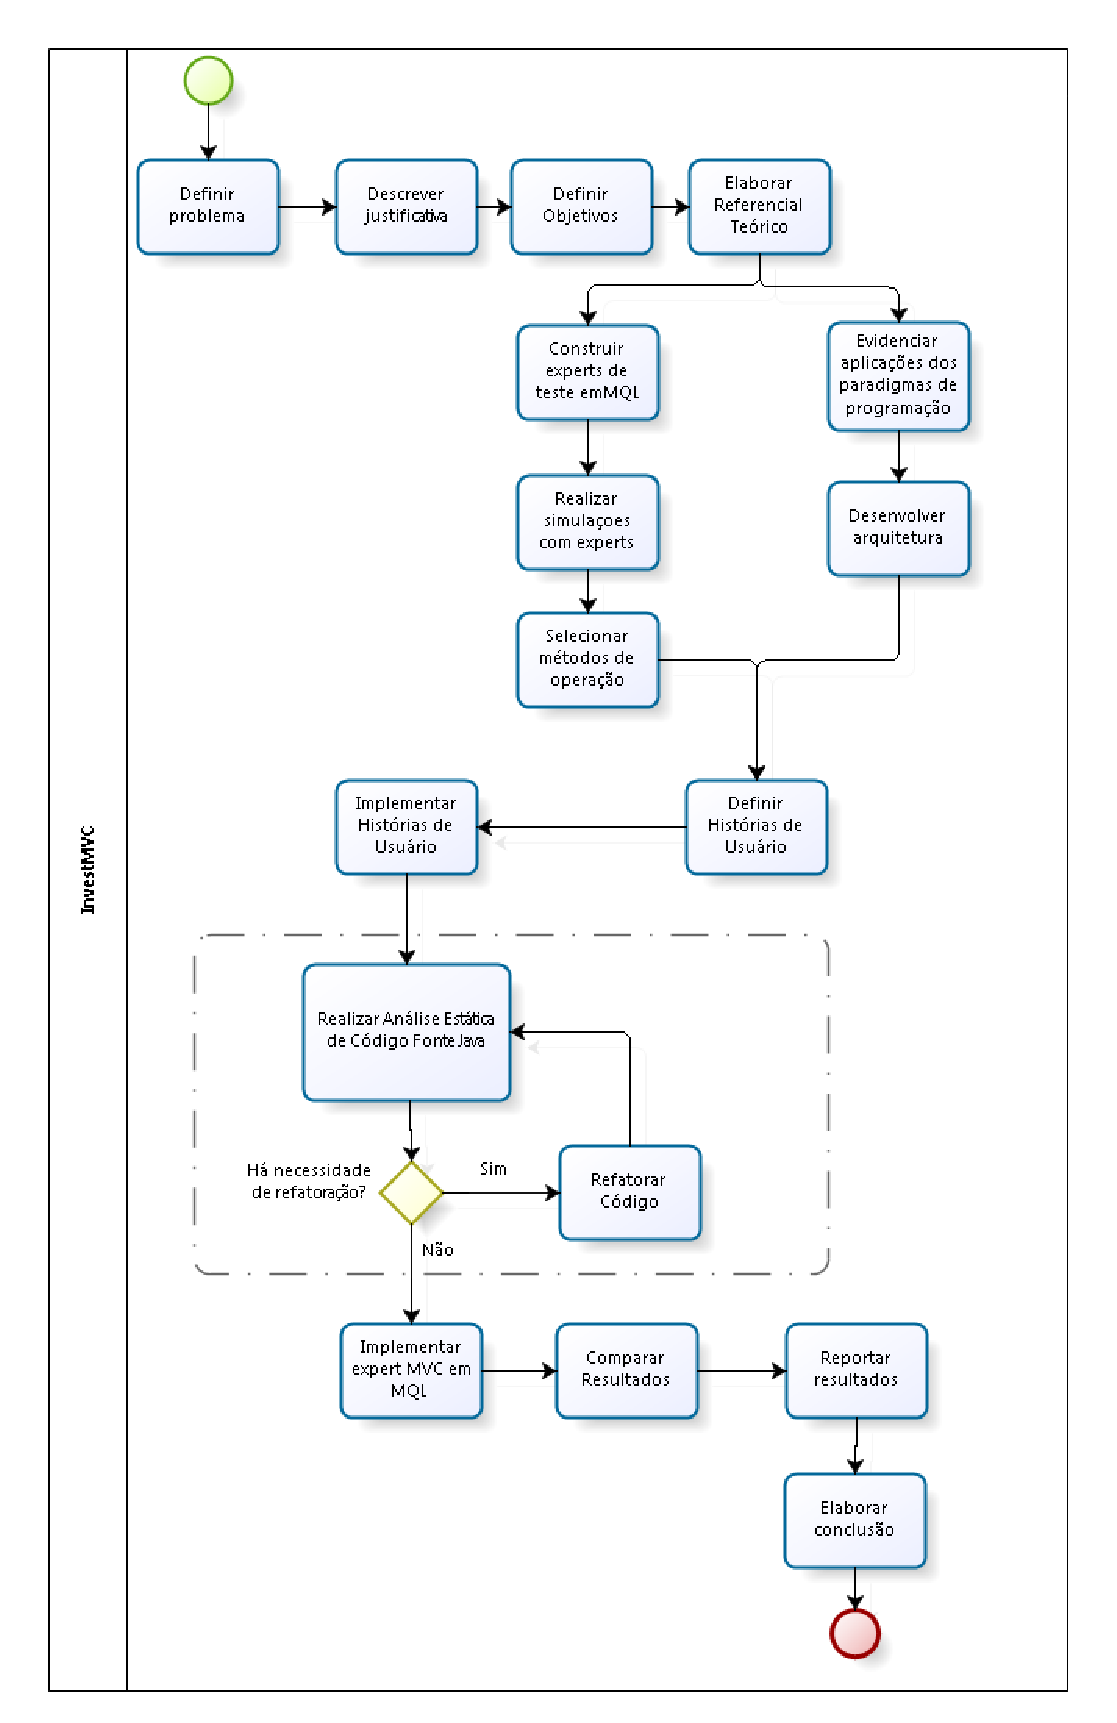
\includegraphics[width=0.7\textwidth]{figuras/metodologiaTCC}
\caption{Atividades da Pesquisa.} 
\label{metodologia}
\end{figure}

\subsection{Descrição dos Objetivos das Atividades de Pesquisa}

A Tabela \ref{atividadeMetologia}  evidencia cada atividade da pesquisa e o objetivo de cada atividade.

\begin{center}
\begin{longtable}{| p{8cm} | p{8cm} |}
\caption{Atividades da pesquisa} \\
\hline
\textbf{Atividade} & \textbf{Objetivo} \\ \hline
\endfirsthead
\multicolumn{2}{c}%
{\tablename\ \thetable\ -- \textit{Continuação da página anterior}} \\
\hline
\textbf{Atividade} & \textbf{Objetivo} \\ \hline
\endhead
\hline \multicolumn{2}{c}{\textit{Continuação na próxima página}} \\
\endfoot
\hline
\endlastfoot
	Definir problema & Definir o problema de pesquisa do trabalho.\\ \hline
	Descrever justificativa & Com base no problema de pesquisa, deve-se justificar a relevância do trabalho proposto.\\ \hline
	Elaborar referencial teórico & Com base na literatura, descrever os conceitos chaves como Contexto Financeiro, Paradigmas de Programação e Qualidade de Software.\\ \hline
	Construir \textit{experts} em mql & Implementar \textit{expert} Fibonacci.mql, MinimosQuadrados.mql, CorrelacaoLinear.mql, Estocastico.mql, MediaMovel.mql. \\ \hline
	Realizar simulação com \textit{experts} & Definir critérios de entrada e saída para cada \textit{expert} e realizar a simulação de cada \textit{expert} no Mercado de Moedas durante o perído de 2 anos (agosto 2012-2014).\\ \hline
	Selecionar métodos de operação & Selecionar os métodos (Fibonacci, Mínimos Quadrados, Correlação Linear, Estocástico ou Média Móvel) que obtiverem lucro durante o período de simulação.\\ \hline
	Evidenciar aplicações dos paradigmas de programação & Evidenciar aplicações dos paradigmas: Funcional, Lógico, Estruturado e Multiagentes.\\ \hline
	Desenvolver arquitetura & Desenvolver a arquitetura do software InvestMVC no intuito de evidenciar decisões sobre a organização do sistema.\\ \hline
	Definir Histórias de Usuário & Definir o conjunto de funcionalidades e pontuar cada História, seguindo a sequência de Fibonacci para realizar a pontuação.\\ \hline
	Implementar Histórias de Usuário & Desenvolver as Histórias de Usuário que foram definidas.\\ \hline
	Realizar Análise Estática de código-fonte & Realizar a análise estática de código-fonte para aferir o nível de qualidade do  software InvestMVC.\\ \hline
	Implementar \textit{expert} em MQL & Implementar toda a lógica do software InvestMVC em linguagem MQL.\\ \hline
	Comparar resultados monetários entre o \textit{expert} MQL e o software InvestMVC & Comparar os resultados monetários do \textit{expert} em MQL com o software InvestMVC durante um tempo a se determinado de operação.\\ \hline
	Reportar resultados & Registrar os resultados da comparação do desempenho do software InvestMVC e do \textit{expert} em MQL.\\ \hline
	Elaborar conclusões & Desenvolver as conclusões do trabalho.
\label{atividadeMetologia}
\end{longtable}
\end{center}

O \textit{backlog} gerado com as histórias de usuário encontra-se no Apêndice A - Histórias de Usuário.

\section{Cronograma}

A Tabela \ref{cronograma} mostra quais foram as atividades em cada Sprint e a duração da mesma. O cronograma detalhado encontra-se no Apêndice B - Cronograma InvestMVC.

\begin{center}
\begin{longtable}{  | p{2cm} | p{8cm} | p{2cm}| p{2cm} |}
\caption{Cronograma simplificado} \\
\hline
\textbf{Sprint} & \textbf{Atividades} & \textbf{Data de início} & \textbf{Data de finalização}\\ \hline
\endfirsthead
\multicolumn{4}{c}%
{\tablename\ \thetable\ -- \textit{Continuação da página anterior}} \\
\hline
\textbf{Sprint} & \textbf{Atividades} & \textbf{Data de início} & \textbf{Data de finalização} \\ \hline
\endhead
\hline \multicolumn{4}{c}{\textit{Continuação na próxima página}} \\
\endfoot
\hline
\endlastfoot
    
    Sprint 1 & \begin{enumerate}
    \item Construir introdução
    \item Implementar Métodos Numéricos
    \end{enumerate} & 10/08/2014 & 31/08/2014\\ \hline
    
    Sprint 2 & \begin{enumerate}
    \item Construir Referencial Teórico Paradigmas de Programação
    \item Adaptar Métodos Numéricos
    \item Prototipar View Projeto
    \item Construir Referencial Teórico Métodos Numéricos
    \end{enumerate} & 01/09/2014 & 15/09/2014\\ \hline
    
    Sprint 3 & \begin{enumerate}
    \item Refinar Referencial Teórico Paradigmas
    \item Construir Referencial Teórico de Contexto Financeiro
    \item Revisar Referencial Teórico Métodos Numéricos
    \end{enumerate} & 16/09/2014 & 30/09/2014\\ \hline
    
    Sprint 4 & \begin{enumerate}
    \item Realizar estudo de caso dos Métodos de Operação
    \item Revisar Referencial Teórico Contexto Financeiro
    \item Desenvolver \textit{experts} em MQL4
    \end{enumerate} & 01/10/2014 & 15/10/2014\\ \hline
    
    Sprint 5 & \begin{enumerate}
    \item Descrever Metodologia de Pesquisa
    \item Realizar estudo de caso dos  Métodos de Operação
    \item Evidenciar Aplicações Paradigmas de Programação
    \end{enumerate} & 16/10/2014 & 31/10/2014\\ \hline
    
    Sprint 6 & \begin{enumerate}
    \item Definir Backlog de Histórias de Usuário
    \item Verificar Qualidade de código-fonte
    \end{enumerate} & 01/11/2014 & 10/11/2014\\ \hline

    Sprint 7 & \begin{enumerate}
    \item Implementar US1
    \item Implementar US5
    \item Implementar US11
    \item Implementar US12
    \end{enumerate} & 09/03/2015 & 24/03/2015\\ \hline

    Sprint 8 & \begin{enumerate}
    \item Implementar US2
    \item Implementar US3
    \item Implementar US4
    \item Implementar US17
    \end{enumerate} & 25/03/2015 & 15/04/2015\\ \hline

    Sprint 9 & \begin{enumerate}
    \item Implementar US18
    \item Implementar US7
    \item Implementar US19
    \item Verificar Qualidade de código-fonte
    \end{enumerate} & 16/04/2015 & 07/05/2015\\ \hline

    Sprint 10 & \begin{enumerate}
    \item Implementar US20
    \item Implementar US21
    \item Implementar US22
    \end{enumerate} & 08/05/2015 & 29/05/2015\\ \hline

    Sprint 11 & Contingência & 30/05/2015 & 19/05/2015

\label{cronograma}
\end{longtable}
\end{center}

\section{Execução da Pesquisa}

Scrum é uma metodologia de desenvolvimento fundada na teoria do controle de processos empíricos. O empirismo afirma que conhecimento vem da experiência. As decisões são tomadas com base na experiência em que se tem de um determinado assunto. Scrum emprega uma abordagem iterativa e incremental para otimizar a previsibilidade e controle de riscos da execução de um projeto. Existem três pilares que sustentam qualquer implementação de controle de processos empíricos: transparência, inspeção e adaptação \cite[pág.~4]{schwaber2013}.

Neste trabalho, vertentes defendidas pelo Scrum foram adaptadas e incorporadas à metodologia de pesquisa. Os produtos de  trabalho foram alocados e desenvolvidos em Sprints (intervalo de tempo de 1 a 4 semanas). Durante a execução de cada Sprint, foram realizadas as adaptações necessárias para que os produtos de trabalho fossem produzidos com sucesso.

Na Sprint 1, foi construída a proposta de trabalho e foi implementado os Métodos Matemáticos em linguagem C que serviram como prova de conceito para viabilizar o desenvolvimento do trabalho.

Na Sprint 2, foi construído o referencial teórico dos Métodos Matemáticos e paradigmas de programação. Também foi feito um protótipo do software InvestMVC para evidenciar como seria a \textit{view} da ferramenta com a dinâmica de construir um robô, selecionar e ativar um robô.

Na Sprint 3, foram refinados o referencial teórico feito na Sprint 2 e foi construído o referencial teórico do Contexto Financeiro.

Na Sprint 4, foi definida a metodologia de pesquisa e foram descritas algumas aplicações dos paradigmas de programação.

A Sprint 5 foi utilizada para atender os resultados do primeiro objetivo específico do trabalho (i.e. selecionar os Métodos Matemáticos do software InvestMVC). Para isso, foram utilizadas simulações para os métodos de fibonacci, correlação de Pearson, mínimos quadrados, média móvel e estocástico. Para realizar essas simulações, foram construídos \textit{experts} para cada método matemático. Ao final das simulações, foram selecionados os Métodos Matemáticos de correlação de Pearson, fibonacci e mínimos quadrados.

A Sprint 6 foi utilizada para definir o backlog de Histórias de Usuário. As pontuações de cada História foram definidas com base na complexidade de cada uma. Nessa Sprint, também foi realizada a análise estática de código-fonte do paradigma estruturado e obteve-se uma qualidade de código aceitável.

Na Sprint 7, foi definido que seriam desenvolvido as Histórias de Usuário US1 (Agente Correlação Linear), US5 (Agente gestor), US11(ativar \textit{expert}) e US12 (desativar \textit{expert}). Não foi possível terminar, as Histórias US11 e US12 nessa Sprint.

Na Sprint 8, foram desenvolvidas as Histórias US11 e US12 que não haviam sido terminadas na Sprint anterior. Foram desenvolvidas as Histórias de Usuário US4 (Agente Tendência), US2 (Agente Fibonacci) e US17 (método Fibonacci em linguagem Haskell). Com essas Histórias de Usuários implementadas, já foi possível disponibilizar a primeira versão do software InvestMVC.

A Sprint 9 estava prevista para construir a US18 (método de Mínimos Quadrados em linguagem Haskell) e US7 (acompanhar retorno financeiro). Entretanto, foi refeito o planejamento dessa Sprint para atender demandas com maior prioridade. A Sprint 9 foi destinada para realizar alguns ajustes metodológicos e escrever os resultados obtidos com as Histórias de Usuário desenvolvidas nas Sprints anteriores. Além disso, foi elaborado um formulário para obter o \textit{feedback} dos usuários que começaram a utilizar a primeira versão da ferramenta na Sprint anterior. Infelizmente, foi detectado que os resultados obtidos na execução dos códigos feitos em linguagem C e em linguagem Haskell não forneciam resultados similares. Como consequência nem todos os resultados previstos foram documentados nessa Sprint.

Devido aos acontecimentos ocorridos na Sprint 9, a Sprint 10 foi totalmente replanejada, criando uma nova Sprint para alocar as atividades que eram da Sprint 10.

Na Sprint 10, foi detectada a necessidade de excluir a US20 (retirar da base de conhecimento). Foi realizada a análise estática de código-fonte dos paradigmas multiagente e estruturado. Os resultados da qualidade de código e os resultados não documentados da Sprint anterior foram feitos.

Na Sprint 11, foi construída a US22 (\textit{expert} no componente MQL), permitindo a integração entre o componente MQL e Multiagente \textit{expert}. Após colocar o software InvestMVC para rodar, percebeu-se que o software teve problemas, com "mortes" de alguns agentes. Esse problema foi contornado e o software voltou a rodar e coletar histórico das operações financeiras. Sendo assim, uma versão estável do software InvestMVC ficou pronta.

\section{Planejamento do estudo de caso}

Esta seção descreve o planejamento para seleção dos Métodos Matemáticos e comparação dos valores monetários do software InvestMVC com os \textit{experts} tradicionais implementados em linguagem MQL que são, respectivamente, os objetivos específicos 1 (um) e 5 (cinco) deste trabalho. Os demais objetivos específicos são produtos de trabalho que dão suporte ao desenvolvimento do software InvestMVC e não possuem um rigor metodológico rigoroso com projeto, coleta e análise dos dados, por exemplo. Na seção Execução da pesquisa, é evidenciado com clareza como foi a dinâmica para que todos os objetivos específicos deste trabalho fossem alcançados.

 O planejamento deste estudo de caso é uma adaptação do template de protocolo de estudo de caso presente no Anexo A - Protocolo de estudo de caso \cite{brereton}.

\subsection{Estudos Anteriories}
Não foi encontrado na literatura vigente nenhum estudo que compare os resultados monetários de Métodos Matemáticos implementados em linguagem MQL ou que defina quais são os métodos aceitáveis para serem implementados em um software multiparadigma para operar no Mercado de Moedas. Também não foi encontrado nenhum estudo que compare os resultados monetários de um software desenvolvido através de uma abordagem multiparadigma de programação com um software implementado em um único paradigma de programação.

\subsection{Projeto do estudo de caso}
Nesta seção é definido o projeto do estudo de caso para atender os objetivos específicos deste trabalho.

\subsubsection{Projeto para seleção dos Métodos Matemáticos}
O objetivo do projeto do estudo de caso da seleção dos Métodos Matemáticos foi definir os valores das variáveis atreladas as operações no Mercado de Moedas para que fosse possível selecionar os métodos a serem implementados no software InvestMVC.

Para se selecionar os métodos de operação no Mercado de Moedas do software InvestMVC, foi definido as seguintes variá¡veis e seus devidos valores:

\begin{itemize}
\item Alavancagem com valor de 0.25;
\item Conta de simulação com valor inicial de 3.000 USD;
\item Margem de negociação/alavancagem da conta igual a 1:500;
\item \textit{Stop loss} e \textit{take profit} definido em 500 pontos;
\item\textit{Experts} programados em linguagem MQL4;
\item Simulaçãoo realizada no mesmo período de tempo (Agosto de 2012 à Agosto de 2014);
\item Simulações realizadas na mesma máquina e mesmo sistema operacional;
\end{itemize}

\subsubsection{Projeto de comparação dos resultados financeiros}

Para realizar a comparação dos valores monetários do software InvestMVC com o software tradicional em linguagem MQL, foram definidas variáveis de operação iguais para ambos os produtos de software:

\begin{itemize}
\item Sistema operacional Linux (Ubuntu 12.04 ou superior);
\item Alavancagem com valor de 0.1;
\item Conta de simulação com valor inicial de 1.000 USD;
\item Margem de negociação/alavancagem da conta igual a 1:500;
\item \textit{Stop loss} definidos de acordo com a estratégia do método Mínimos Quadrados;
\item \textit{Take profit} definidos de acordo com a estratégia do método Mínimos Quadrados;
\item Quantidade de \textit{candles} em 55;
\item Critério de entrada da Correlação de Pearson maior ou igual a 0.9;
\item Critério de entrada de Fibonacci em 0.38;
\item Gráfico de negociação euro-dólar;
\item Tipo de gráfico de negociação de 5 minutos;
\item Início das negociações às 18:00 h de todo domingo;
\item Fim das negociações às 18:00 h de toda sexta-feira;
\item Tempo de negociação por dia de 24 horas;
\end{itemize}

\subsection{Coleta de dados}
Esta seção define os atributos de coleta de dados para a seleção dos Metodos Matemáticos e comparação dos resultados financeiros do software InvestMVC com o software tradicional implementado em linguagem MQL.

\subsubsection{Coleta de dados para seleção dos Métodos Matemáticos}
Os dados coletados para seleção dos Métodos Matemáticos são: cotações do par de moedas euro-dólar (preço da cotação de abertura e fechamento); data do início e fim da ordem; tipo da ordem (compra ou venda); \textit{stop loss}; \textit{take profit} e resultado da operação (lucro ou prejuízo). Todos esses dados são fornecidos pelo histórico da ferramenta MetaTrader.

A ferramenta MetaTrader já fornece um relatório completo e detalhado do rendimento dos métodos que são colocados em simulação. Portanto, não tem necessidade de fazer um plano para armazenamento dos dados coletados. Os resultados das simulações (gráficos e relatórios de desempenho), são salvos em arquivos com extensões csv ou html.

\subsubsection{Coleta de dados para comparação dos resultados financeiros}
Da mesma forma que a seleção dos Métodos Matemáticos, os dados coletados para comparação dos resultados financeiros são: cotações do par de moedas euro-dólar (preço da cotação de abertura e fechamento); data do início e fim da ordem; tipo da ordem (compra ou venda); \textit{stop loss}; \textit{take profit} e resultado da operação (lucro ou prejuízo). Esses resultados também são oferecidos nos históricos gerados pela ferramenta MetaTrader.

Os históricos dos resultados financeiros são salvos em planilhas ou em arquivos com extensão html. Sendo assim, é possível armazenar esses dados para fazer análises dos valores monetários extraídos dos históricos das operações.

\subsection{Análise dos dados}
O critério para seleção dos Métodos Matemáticos e comparação dos valores monetários é o rendimento sob o capital investido. Os demais dados descritos na seção de coleta de dados (como cotações, data de início e fim da ordem), dão suporte e ajuda a explicar o motivo do rendimento financeiro ser maior ou menor de acordo com um valor de investimento. Entretanto, a análise dos demais dados não fazem parte do escopo deste trabalho.

O critério para análise e selação dos Métodos Matemáticos foi o percentual de lucro sob o capital investido. Os Métodos Matemáticos que obtiveram 10\% de lucro sob capital inicial, foram selecionados para serem implementados no software InvestMVC. 

A análise dos resultados monetários é feita com base no histórico das operações. É considerado o resultado da operação (lucro ou prejuízo) como critério para realização da análise.

\subsection{Plano de validação} 
Para que o software InvestMVC realize uma operação de compra ou venda, devem ser realizados cálculos matemáticos pelos paradigmas Estruturado e Funcional. Ambos paradigmas realizam os mesmos cálculos para validar os resultados dos Métodos Matemáticos para realização das operações. 

O paradigma Multiagente é responsável por receber os cálculos dos métodos de Mínimos Quadrados, Fibonacci e Correlação Linear através dos paradigmas Estruturado e Lógico. Feito isso, os resultados fornecidos são validados pelo paradigma Multiagente com um nível erro de acordo com a Tabela \ref{erroMetodos}. O nível de erro foi definido de forma empírica, considerando a complexidade dos cálculos dos Métodos Matemáticos. Quanto maior a complexidade do cálculo matemático, maior foi o valor do nível de erro aceitado.

\begin{center}
\begin{longtable}{| p{8cm} | p{8cm} |}
\caption{Erro aceitável de cada Método Matemático} \\
\hline
\textbf{Método Matemático} & \textbf{Nível de erro para validação} \\ \hline
\endfirsthead
\multicolumn{2}{c}%
{\tablename\ \thetable\ -- \textit{Continuação da página anterior}} \\
\hline
\textbf{Método matemático} & \textbf{Nível de erro para validação} \\ \hline
\endhead
\hline \multicolumn{2}{c}{\textit{Continuação na próxima página}} \\
\endfoot
\hline
\endlastfoot

Correlação Linear & 0.0010\\ \hline
Fibonacci & 0.0001\\ \hline
Mínimos Quadrados & 0.0100

\label{erroMetodos}
\end{longtable}
\end{center}

A Tabela \ref{exemploErro} evidencia possíveis resultados dos Métodos Matemáticos nos paradigmas Estruturado e Funcional e qual deve ser a resposta do paradigma Multiagente, levando em consideração o nível de erro para validação.

\begin{center}
\begin{longtable}{| p{4cm} | p{3cm} | p{3cm} | p{3cm} | p{2cm} |}
\caption{Exemplo de validação do paradigma Multiagente} \\
\hline
\textbf{Método Matemático} & \textbf{Cálculo paradigma Estruturado} & \textbf{Cálculo paradigma Funcional} & \textbf{Nível de erro para validação} & \textbf{Validado pelo paradigma Mutilagente?}\\ \hline
\endfirsthead
\multicolumn{5}{c}%
{\tablename\ \thetable\ -- \textit{Continuação da página anterior}} \\
\hline
\textbf{Método Matemático} & \textbf{Cálculo paradigma Estruturado} & \textbf{Cálculo paradigma Funcional} & \textbf{Nível de erro para validação} & \textbf{Validado pelo paradigma Mutilagente?}\\ \hline
\endhead
\hline \multicolumn{5}{c}{\textit{Continuação na próxima página}} \\
\endfoot
\hline
\endlastfoot

Correlação Linear & 0.9000000 & 0.9100000 & 0.0010 & NÃO\\ \hline
Fibonacci & 0.6182578 & 0.6182577 & 0.0001 & SIM\\ \hline
Mínimos Quadrados & 0.912778 & 0.912779 & 0.0100 & SIM

\label{exemploErro}
\end{longtable}
\end{center}

Como os resultados dos Métodos Matemáticos possui um plano de validação, não é necessário validar os resultados dos valores monetários, pois os mesmos são originados através das operações de compra ou venda, que por sua vez, são realizadas através dos cálculos matemáticos.

\subsection{Limitações do Estudo}

A linguagem MQL4 não possui suporte para teste unitário. Portanto, os \textit{experts} tradicionais programados para este estudo de caso, não possuem testes automatizados. A linguagem MQL4 também não possui nenhuma ferramenta para realizar uma análise estática de código. Logo, não é possível determinar o nível de qualidade de código-fonte dos códigos desenvolvidos.

O software InvestMVC só roda no sistema operacional Linux e utiliza o Wine para rodar o MetaTrader, pois o MetaTrader só roda no sistema operacional Windows. Portanto, nada garante que o Wine não trave em algum momento e faça com que o software InvestMVC deixe de realizar uma operação de compra ou venda.

O simulador do MetaTrader possui código- fonte fechado. Portanto, não foi possível realizar nenhuma adaptação da ferramenta para auxilar no desenvolvimento do software InvestMVC. Por exemplo, a ferramenta MetaTrader fornece ao usuário o histórico de operações, mas não é possível o software InvestMVC utilizar esse histórico. Nesse caso, tem que ser implementado o código para calcular o histórico dos resultados monetários.